\section{A model-checker for process models\label{section:tool-model-checker}}

Our model-checker for guarded hMSC extends the compositional model-checking technique presented in \cite{Giannakopoulou:2003}. The latter allows model-checking LTS state machines against FLTL safety properties. Our model-checker extends this in two directions:
\begin{itemize}
\item it allows either a g-hMSC or a g-LTS as input; in the former case, the g-hMSC is immediately derived as a g-LTS with the algorithm described in Section \ref{subsection:from-ghmsc-to-glts};
\item the main algorithm compose g-LTS instead of LTS, as explained in Section \ref{subsection:glts-operators}. 
\end{itemize}

The model-checking technique is illustrated on Fig.~\ref{image:model-checking-technique}. Roughly, it consists in searching for an error state in the the state-space defined by a composition of g-LTSs: one for the model, one for each fluent and one for the satefy property.

\begin{figure}[H]
\centering\scalebox{.525}{
  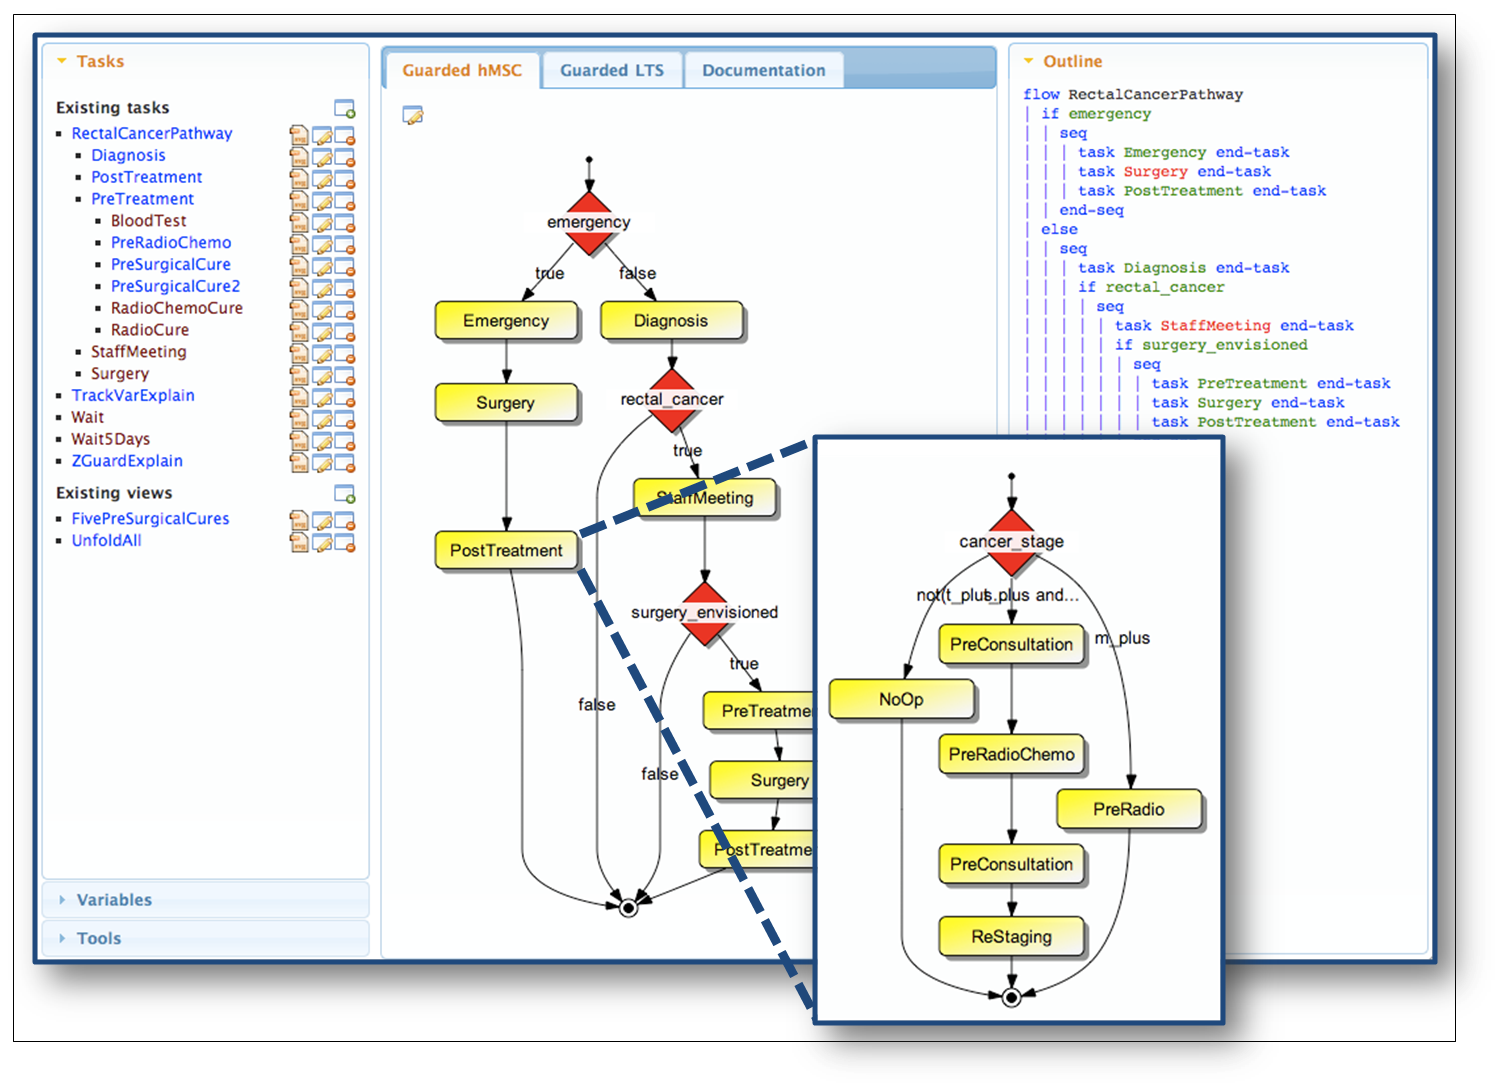
\includegraphics[trim=5mm 10mm 10mm 5mm, clip]{src/7-tool-support/images/gisele-tool}}
  \caption{Architecture of the g-hMSC model checker\label{image:model-checking-technique}}
\end{figure}

The logical architecture of our model-checker is depicted in Fig.~\ref{image:model-checker}. Its implementation mostly relies on three main modules:

\begin{figure}[H]
\centering\scalebox{.525}{
  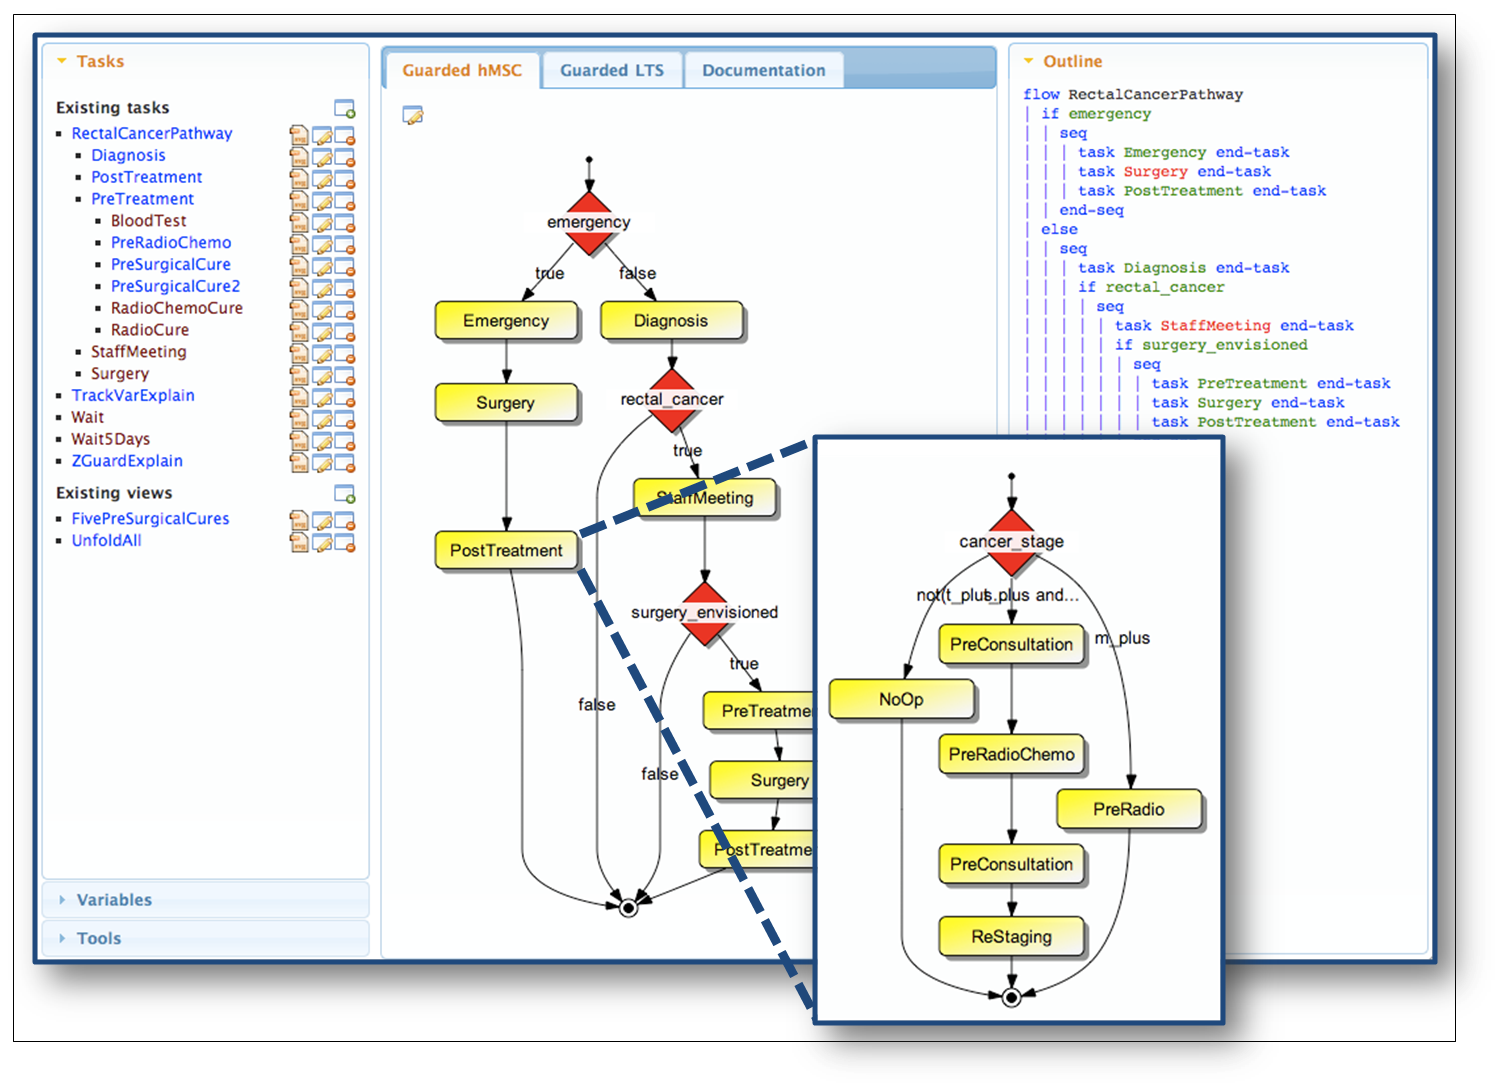
\includegraphics[trim=5mm 10mm 10mm 5mm, clip]{src/7-tool-support/images/gisele-tool}}
  \caption{Architecture of the g-hMSC model checker\label{image:model-checker}}
\end{figure}

\begin{description}
\item[Guarded LTS] The first module is an implementation of guarded LTS, notably the composition operator described in Section~\ref{subsection:glts-operators}. This module reuses our abstract automaton toolkit, namely Jail (which stands for Java Automaton and Induction Library) and a library called JavaBDD\footnote{available at http://javabdd.sourceforge.net/ (last retrieved 2011-08-25)} for efficiently manipulating Boolean formula through Binary Decision Diagrams \cite{Bryant:1986}.

Jail implements an automaton data structure together with standard algorithms:  minimization, determinization, composition, etc. It has been designed as a fairly abstract library in that it allows states and edges of automata to be decorated with any \emph{(key,value)} pairs. Jail algorithms can be configured to perform specific operations on such decorations when manipulating states and edges. As standard automaton algorithms often compute and/or merge sets of states and edges, Jail provides built-in implementations of aggregation operators (sum, avg, min, max, set union, set intersection, and so on).

JavaBDD is used for implementing guards efficiently. A particular configuration of the composition operator in Jail yields the g-LTS composition operator defined in Section~\ref{subsection:glts-operators}. In particular, a specific aggregation operator for edges uses BDDs for implementing the conjuction of guards.

\item[FLTL] This second module implements fluents and FLTL temporal properties with the use of the LTL2Buchi\footnote{available at http://ti.arc.nasa.gov/profile/dimitra/projects-tools/ (last retrieved 2011-08-25)} library \cite{Giannakopoulou:2002}. 

LTL2Buchi is used to parse LTL specifications and translates them to B\"uchi automata. Our FLTL module interfaces with LTL2Buchi and translates its B\"uchi automata in our g-LTS. It also translates fluent definitions to g-LTS as explained in Section~\ref{subsection:from-glts-to-lts}.

\item[Guarded hMSC] This structural module implements Guarded hMSC. It mostly consists in the implementation of a graph made of tasks and decision nodes and an API to build them programmatically.
\end{description}

The main module of the model checker provides an API for deriving guarded LTS and LTS from guarded hMSC as well as model-checking them. 
